\documentclass[]{beamer}\usepackage[]{graphicx}\usepackage[]{color}
%% maxwidth is the original width if it is less than linewidth
%% otherwise use linewidth (to make sure the graphics do not exceed the margin)
\makeatletter
\def\maxwidth{ %
  \ifdim\Gin@nat@width>\linewidth
    \linewidth
  \else
    \Gin@nat@width
  \fi
}
\makeatother

\definecolor{fgcolor}{rgb}{0.345, 0.345, 0.345}
\newcommand{\hlnum}[1]{\textcolor[rgb]{0.686,0.059,0.569}{#1}}%
\newcommand{\hlstr}[1]{\textcolor[rgb]{0.192,0.494,0.8}{#1}}%
\newcommand{\hlcom}[1]{\textcolor[rgb]{0.678,0.584,0.686}{\textit{#1}}}%
\newcommand{\hlopt}[1]{\textcolor[rgb]{0,0,0}{#1}}%
\newcommand{\hlstd}[1]{\textcolor[rgb]{0.345,0.345,0.345}{#1}}%
\newcommand{\hlkwa}[1]{\textcolor[rgb]{0.161,0.373,0.58}{\textbf{#1}}}%
\newcommand{\hlkwb}[1]{\textcolor[rgb]{0.69,0.353,0.396}{#1}}%
\newcommand{\hlkwc}[1]{\textcolor[rgb]{0.333,0.667,0.333}{#1}}%
\newcommand{\hlkwd}[1]{\textcolor[rgb]{0.737,0.353,0.396}{\textbf{#1}}}%
\let\hlipl\hlkwb

\usepackage{framed}
\makeatletter
\newenvironment{kframe}{%
 \def\at@end@of@kframe{}%
 \ifinner\ifhmode%
  \def\at@end@of@kframe{\end{minipage}}%
  \begin{minipage}{\columnwidth}%
 \fi\fi%
 \def\FrameCommand##1{\hskip\@totalleftmargin \hskip-\fboxsep
 \colorbox{shadecolor}{##1}\hskip-\fboxsep
     % There is no \\@totalrightmargin, so:
     \hskip-\linewidth \hskip-\@totalleftmargin \hskip\columnwidth}%
 \MakeFramed {\advance\hsize-\width
   \@totalleftmargin\z@ \linewidth\hsize
   \@setminipage}}%
 {\par\unskip\endMakeFramed%
 \at@end@of@kframe}
\makeatother

\definecolor{shadecolor}{rgb}{.97, .97, .97}
\definecolor{messagecolor}{rgb}{0, 0, 0}
\definecolor{warningcolor}{rgb}{1, 0, 1}
\definecolor{errorcolor}{rgb}{1, 0, 0}
\newenvironment{knitrout}{}{} % an empty environment to be redefined in TeX

\usepackage{alltt}
%\documentclass[handout]{beamer}
%\usepackage[dvips]{color}
%\usepackage{beamerprosper}
\usepackage{graphicx}
%\usepackage{psfrag, pstricks}
\usepackage{amsmath,amssymb,array,comment,eucal}
\usepackage{xcolor}
\definecolor{beamer@blendedblue}{RGB}{86,155,189}
\definecolor{myblue}{RGB}{12,76,138}
\setbeamercolor{structure}{fg=myblue}
\definecolor{Ftitle}{RGB}{12,76,138}
\definecolor{Descitem}{RGB}{238,238,244}
\definecolor{StdTitle}{RGB}{12,76,138}
\definecolor{StdBody}{RGB}{213,24,0}
\definecolor{StdBody}{RGB}{213,24,0}

\definecolor{AlTitle}{RGB}{255, 190, 190}
\definecolor{AlBody}{RGB}{213,24,0}

\definecolor{ExTitle}{RGB}{201, 217, 217}
\definecolor{ExBody}{RGB}{213,24,0}

\setbeamercolor{frametitle}{fg = Ftitle}
\setbeamercolor{title}{fg = Ftitle}
\setbeamercolor{item}{fg = Ftitle}
\setbeamercolor{subitem}{fg = Ftitle}
\setbeamercolor{subsubitem}{fg = Ftitle}
\setbeamercolor{description item}{fg = myblue}
\setbeamercolor{titlelike}{fg=myblue}

%$Id: macros.tex,v 1.2 2006/02/13 14:23:55 rlw Exp rlw $
\newcommand{\Lmea}{{\cal L}} 
\newcommand{\scale}{\bflambda} 
\newcommand{\Scale}{\bfLambda} 
\newcommand{\bfscale}{\bflambda} 
\newcommand{\mean}{\bfchi}
\newcommand{\loc}{\bfchi}
\newcommand{\bfmean}{\bfchi}
\renewcommand{\k}{g}
\newcommand{\Gen}{{\cal G}}
\newcommand{\eps}{\epsilon}

\newcommand{\ind}{\mathrel{\mathop{\sim}\limits^{\mathit{ind}}}}
\newcommand{\iid}{\mathrel{\mathop{\sim}\limits^{\mathit{iid}}}}
\newcommand{\dis}{\mathrel{\mathop{=}\limits^{d}}}
\newcommand{\sgn}{\mathop{\rm sgn}}
\newcommand{\cmp}{h}
\newcommand{\dbdo}{d\beta ~ d\omega}
\newcommand{\real}{{\mathbb{R}}}
\newcommand{\Ber}{\mbox{\rm Ber}}
\newcommand{\GP}{\mbox{\rm GP}}
\newcommand{\SaS}{\text{S$\alpha$S}}
\newcommand{\RA}{{\real \times A}}
\newcommand{\RK}{{\real \times K}}
\newcommand{\RO}{{\real \times \Omega}} 
\newcommand{\RS}{{\bbR \times \LamS}}
  \newcommand{\set}[1]{\left\{#1\right\}}
  \newcommand{\bet}[1]{\left[#1\right]}
  \newcommand{\cet}[1]{\left(#1\right)}
%  \renewcommand{\half}{{\scriptstyle\frac12}}
\newcommand{\subA}{(\eps_1 < \beta \le \eps_2) \times \LamS}
 \newcommand{\uu}{{\big(\scale(x - \loc)\big)}}
 \newcommand{\uuj}{{\big(\scale_j(x-\loc_j)\big)}}
 \newcommand{\bbT}{{\mathbb{T}}}
 \newcommand{\ui}{{[0,1)}}
 \newcommand{\spq}[1]{\left|#1\right|^s_{pq}}
 \newcommand{\spqper}[1]{\left|#1\right|^{s\,*}_{pq}}
 \newcommand{\sspqper}[1]{\left\|#1\right\|^{s\,*}_{pq}}
 \newcommand{\sspq}[1]{\left\|#1\right\|^s_{pq}}    % Besov semi-norm
 \newcommand{\qp}[1]  {\left\|#1\right\|^q_p}         % Hilbert-space norm
 \newcommand{\qper}[1]{\left\|#1\right\|^{*\,q}_p}  % Periodic HS norm
 

\newcommand{\bbW}{{\mathbb{W}}}
\newcommand{\bbB}{{\mathbb{B}}}
\newcommand{\Sob}{{\ensuremath{\bbW^s_2}}}
\newcommand{\Besov}{{\ensuremath{\bbB^s_{pq}}}}
\newcommand{\Besper}{{\ensuremath{\bbB^{s\,*}_{pq}}}}
\newcommand{\Sobx}[1]{{\bbW^{#1}_2}}
\newcommand{\Besovx}[1]{{\bbB^{#1}_2}}
\newcommand{\SN}[1]{\|{#1}\|_\Sob}
% MATH LETTER DEFINITIONS
\newcommand{\Levy}{L{\'e}vy}
\newcommand{\nmathbf}{\bm}
\newcommand{\tabb}[1]{\hspace*{#1\parindent}}
%\newcommand{\G}{{g}}    % Really the same as \GB
\newcommand{\g}{{\phi}} %\newcommand{\g}{{g}}
\newcommand{\GB}{{g}}  
% Roman math Bold face 


\def\bfA{\nmathbf A}
\def\bfB{\nmathbf B}
\def\bfC{\nmathbf C}
\def\bfD{\nmathbf D}
\def\bfE{\nmathbf E}
\def\bfF{\nmathbf F}
\def\bfG{\nmathbf G}
\def\bfH{\nmathbf H}
\def\bfI{\nmathbf I}
\def\bfJ{\nmathbf J}
\def\bfK{\nmathbf K}
\def\bfL{\nmathbf L}
\def\bfM{\nmathbf M}
\def\bfN{\nmathbf N}
\def\bfO{\nmathbf O}
\def\bfP{\nmathbf P}
\def\bfQ{\nmathbf Q}
\def\bfR{\nmathbf R}
\def\bfS{\nmathbf S}
\def\bfT{\nmathbf T}
\def\bfU{\nmathbf U}
\def\bfV{\nmathbf V}
\def\bfW{\nmathbf W}
\def\bfX{\nmathbf X}
\def\bfY{\nmathbf Y}
\def\bfZ{\nmathbf Z}

\def\bfa{\nmathbf a}
\def\bfb{\nmathbf b}
\def\bfc{\nmathbf c}
\def\bfd{\nmathbf d}
\def\bfe{\nmathbf e}
\def\bff{\nmathbf f}
\def\bfg{\nmathbf g}
\def\bfh{\nmathbf h}
\def\bfi{\nmathbf i}
\def\bfj{\nmathbf j}
\def\bfk{\nmathbf k}
\def\bfl{\nmathbf l}
\def\bfm{\nmathbf m}
\def\bfn{\nmathbf n}
\def\bfo{\nmathbf o}
\def\bfp{\nmathbf p}
\def\bfq{\nmathbf q}
\def\bfr{\nmathbf r}
\def\bfs{\nmathbf s}
\def\bft{\nmathbf t}
\def\bfu{\nmathbf u}
\def\bfv{\nmathbf v}
\def\bfw{\nmathbf w}
\def\bfx{\nmathbf x}
\def\bfy{\nmathbf y}
\def\bfz{\nmathbf z}


\def\bfalpha  {\nmathbf \alpha}
\def\bfbeta   {\nmathbf \beta}
\def\bfgamma  {\nmathbf \gamma}
\def\bfdelta  {\nmathbf \delta}
\def\bfepsilon{\nmathbf \epsilon}
\def\bfvareps {\nmathbf \varepsilon}
\def\bfzeta   {\nmathbf \zeta}
\def\bfeta    {\nmathbf \eta}
\def\bftheta  {\nmathbf \theta}
\def\bfiota   {\nmathbf \iota}
\def\bfkappa  {\nmathbf \kappa}
\def\bflambda {\nmathbf \lambda}
\def\bfmu     {\nmathbf \mu}
\def\bfnu     {\nmathbf \nu}
\def\bfxi     {\nmathbf \xi}
\def\bfomicron{\nmathbf \omicron}
\def\bfpi     {\nmathbf \pi}
\def\bfrho    {\nmathbf \rho}
\def\bfsigma  {\nmathbf \sigma}
\def\bftau    {\nmathbf \tau}
\def\bfupsilon{\nmathbf \upsilon}
\def\bfphi    {\nmathbf \phi}
\def\bfpsi    {\nmathbf \psi}
\def\bfchi    {\nmathbf \chi}
\def\bfomega  {\nmathbf \omega}
\newcommand{\nubw}{{\tilde\nu}}  % no longer red!
\def\bfAlpha  {\nmathbf \Alpha}
\def\bfBeta   {\nmathbf \Beta}
\def\bfGamma  {\nmathbf \Gamma}
\def\bfDelta  {\nmathbf \Delta}
\def\bfEpsilon{\nmathbf \Epsilon}
\def\bfZeta   {\nmathbf \Zeta}
\def\bfEta    {\nmathbf \Eta}
\def\bfTheta  {\nmathbf \Theta}
\def\bfIota   {\nmathbf \Iota}
\def\bfKappa  {\nmathbf \Kappa}
\def\bfLambda {\nmathbf \Lambda}
\def\bfMu     {\nmathbf \Mu}
\def\bfNu     {\nmathbf \Nu}
\def\bfXi     {\nmathbf \Xi}
\def\bfOmicron{\nmathbf \Omicron}
\def\bfPi     {\nmathbf \Pi}
\def\bfRho    {\nmathbf \Rho}
\def\bfSigma  {\nmathbf \Sigma}
\def\bfTau    {\nmathbf \Tau}
\def\bfUpsilon{\nmathbf \Upsilon}
\def\bfPhi    {\nmathbf \Phi}
\def\bfPsi    {\nmathbf \Psi}
\def\bfChi    {\nmathbf \Chi}
\def\bfOmega  {\nmathbf \Omega}

% Number math Bold face

\newcommand{\bfzero}{{\nmathbf 0}}
\newcommand{\bfone}{{\nmathbf 1}}

% Estimators

\newcommand{\ttheta}{\tilde{\theta}}
\newcommand{\htheta}{\hat{\theta}}
\newcommand{\tbtheta}{\tilde{\bftheta}}
\newcommand{\hbtheta}{\hat{\bftheta}}
\newcommand{\tomega}{\tilde{\omega}}
\newcommand{\homega}{\hat{\omega}}
\newcommand{\tbomega}{\tilde{\bfomega}}
\newcommand{\hbomega}{\hat{\bfomega}}
\newcommand{\tlambda}{\tilde{\lambda}}
\newcommand{\hlambda}{\hat{\lambda}}
\newcommand{\tblambda}{\tilde{\bflambda}}
\newcommand{\hblambda}{\hat{\bflambda}}


% Calligraphic

\newcommand{\mc}[1]{\ensuremath{\mathcal{#1}}}

\newcommand{\cfA}{\mc{A}}
\newcommand{\cfB}{\mc{B}}
\newcommand{\cfC}{\mc{C}}
\newcommand{\cfD}{\mc{D}}
\newcommand{\cfE}{\mc{E}}
\newcommand{\cfF}{\mc{F}}
\newcommand{\cfG}{\mc{G}}
\newcommand{\cfH}{\mc{H}}
\newcommand{\cfI}{\mc{I}}
\newcommand{\cfJ}{\mc{J}}
\newcommand{\cfK}{\mc{K}}
\newcommand{\cfL}{\mc{L}}
\newcommand{\cfM}{\mc{M}}
\newcommand{\cfN}{\mc{N}}
\newcommand{\cfO}{\mc{O}}
\newcommand{\cfP}{\mc{P}}
\newcommand{\cfQ}{\mc{Q}}
\newcommand{\cfR}{\mc{R}}
\newcommand{\cfS}{\mc{S}}
\newcommand{\cfT}{\mc{T}}
\newcommand{\cfU}{\mc{U}}
\newcommand{\cfV}{\mc{V}}
\newcommand{\cfX}{\mc{X}}
\newcommand{\cfY}{\mc{Y}}
\newcommand{\cfZ}{\mc{Z}}

\newcommand{\bmc}[1]{\ensuremath{\boldsymbol{\mathcal{#1}}}}

\newcommand{\bcfA}{\bmc{A}}
\newcommand{\bcfB}{\bmc{B}}
\newcommand{\bcfC}{\bmc{C}}
\newcommand{\bcfD}{\bmc{D}}
\newcommand{\bcfE}{\bmc{E}}
\newcommand{\bcfF}{\bmc{F}}
\newcommand{\bcfG}{\bmc{G}}
\newcommand{\bcfH}{\bmc{H}}
\newcommand{\bcfI}{\bmc{I}}
\newcommand{\bcfJ}{\bmc{J}}
\newcommand{\bcfK}{\bmc{K}}
\newcommand{\bcfL}{\bmc{L}}
\newcommand{\bcfM}{\bmc{M}}
\newcommand{\bcfN}{\bmc{N}}
\newcommand{\bcfO}{\bmc{O}}
\newcommand{\bcfP}{\bmc{P}}
\newcommand{\bcfQ}{\bmc{Q}}
\newcommand{\bcfR}{\bmc{R}}
\newcommand{\bcfS}{\bmc{S}}
\newcommand{\bcfT}{\bmc{T}}
\newcommand{\bcfU}{\bmc{U}}
\newcommand{\bcfV}{\bmc{V}}
\newcommand{\bcfW}{\bmc{W}}
\newcommand{\bcfX}{\bmc{X}}
\newcommand{\bcfY}{\bmc{Y}}
\newcommand{\bcfZ}{\bmc{Z}}

% Special symbols

\newcommand{\reals}{\mbox{\rm I\kern-.20em R}}
\newcommand{\sreals}{\mbox{\small \rm I\kern-.20em R}}
\newcommand{\LamS}{{\cS^d_+}}

% MATHEMATICAL NOTATION

% Operators

\newcommand{\bg}{\;\bigg\vert\;}
\newcommand{\pr}{\mbox{\rm Pr}}
\newcommand{\D}{\mbox{\rm D}}
\newcommand{\E}{\mbox{\rm E}}
\newcommand{\Mo}{\mbox{\rm Mo}}
\newcommand{\Me}{\mbox{\rm Me}}
\newcommand{\Cov}{\mbox{\rm Cov}}
\newcommand{\Var}{\mbox{\rm Var}}
\newcommand{\Corr}{\mbox{\rm Corr}}
\newcommand{\Q}{\mbox{\rm Q}}

% Distributions
\newcommand{\BeBi}{\mbox{\rm BeBi}}
\newcommand{\Be}{\mbox{\rm Be}}
\newcommand{\Bi}{\mbox{\rm Bi}}
\newcommand{\Br}{\mbox{\rm Br}}
\newcommand{\Ca}{\mbox{\rm Ca}}
\newcommand{\Di}{\mbox{\rm Di}}
\newcommand{\Ex}{\mbox{\rm Ex}}
\newcommand{\Fs}{\mbox{\rm Fs}}
\newcommand{\Ga}{\mbox{\sf G}}
\newcommand{\Ge}{\mbox{\rm Ge}}
\newcommand{\GaGa}{\mbox{\rm GaGa}}
\newcommand{\Hy}{\mbox{\rm Hy}}
\newcommand{\IGa}{\mbox{\rm IGa}}
\newcommand{\IPa}{\mbox{\rm IPa}}
\newcommand{\Lo}{\mbox{\rm Lo}}
\newcommand{\Mu}{\mbox{\rm Mu}}
\newcommand{\N}{\mbox{\rm N}}
\newcommand{\NBi}{\mbox{\rm NBi}}
\newcommand{\NGa}{\mbox{\rm NGa}}
\newcommand{\NWi}{\mbox{\rm NWi}}
\newcommand{\Pa}{\mbox{\rm Pa}}
\newcommand{\Po}{\mbox{\sf P}}
\newcommand{\PoGa}{\mbox{\rm PoGa}}
\newcommand{\Ra}{\mbox{\rm Ra}}
\newcommand{\REx}{\mbox{\rm REx}}
\newcommand{\St}{\mbox{\rm St}}
\newcommand{\Un}{\mbox{\rm Un}}
\newcommand{\Wi}{\mbox{\rm Wi}}

% General Mathematics

\newcommand{\dd}[1]{\,d{#1}}
\newcommand{\barx}{\ensuremath{\bar{x}}}
\newcommand{\comb}[2]{{#1\choose#2}}
\newcommand{\ontop}[2]{{#1\atop#2}}
\newcommand{\h}{{\small\ensuremath{1\over2}}}
\newcommand{\hh}[2]{{\small\ensuremath{#1\over#2}}}

\newcommand{\fn}[1]{\hbox{\textrm{#1}}}
\newcommand{\cred}{\fn{Cr}}
\newcommand\dlim{\mathop{\rm \hbox{$\delta$}lim}}
\newcommand{\goto}{\rightarrow}
\newcommand{\gotoinf}{\rightarrow \infty}

\newcommand{\data}{\ensuremath{\bfx=\{x_1,\ldots,x_n\}}}
\newcommand{\brow}[2]{\ensuremath{\{{#1}_1,\ldots,{#1}_{#2}\}}}
\newcommand{\prow}[2]{\ensuremath{({#1}_1,\ldots,{#1}_{#2})}}

\newcommand{\met}{\thinspace{\rm m}}\newcommand{\km}{\thinspace{\rm km}}
\newcommand{\xbar}{\overline X}%
\newcommand{\xbbar}{\overline{\overline X}}%
\font\ss=cmss12
 \newcommand{\OFP}{(\Omega,\cF,\P)}
 \newcommand{\bbC}{\mathbb{C}}
 \newcommand{\bbF}{\mathbb{F}}
 \newcommand{\bbN}{\mathbb{N}}
 \newcommand{\bbR}{\mathbb{R}}
 \newcommand{\bbX}{\mathbb{X}}
 \newcommand{\bbZ}{\mathbb{Z}}
 \newcommand{\one}[1]{\mathbf{1}_{\{#1\}}}
 \newcommand{\cA}{{\cal A}}
 \newcommand{\cB}{{\cal B}} 
 \newcommand{\cE}{{\cal E}}
 \newcommand{\cF}{{\cal F}}
 \newcommand{\cG}{{\cal G}}
 \newcommand{\cH}{{\cal H}}
 \newcommand{\cM}{{\cal M}}
 \newcommand{\cR}{{\cal R}}
 \newcommand{\cS}{{\cal S}}
 \newcommand{\cT}{{\cal T}}
 \newcommand{\cX}{{\cal X}}
 \newcommand{\cY}{{\cal Y}}
 \newcommand{\cZ}{{\cal Z}}
 \newcommand{\eF}{{\CMcal F}}
 \newcommand{\eG}{{\CMcal G}} 
 \newcommand{\eH}{{\CMcal H}}
 \renewcommand{\P}{{\sf{P}}} 
 \renewcommand{\E}{{\sf{E}}}
 \newcommand{\Ev}{{\sf{Ev}}}%
 \newcommand{\V}{{\sf{V}}} 
 \renewcommand{\Cov}{{\sf{Cov}}}
 %\newcommand{\Be}{\textsf{Be}}
 %\newcommand{\Bi}{\textsf{Bi}}
 %\newcommand{\Ex}{\textsf{Ex}}\newcommand{\Ga}{\textsf{Ga}}
 %\newcommand{\Di}{\textsf{Di}}\newcommand{\Ge}{\textsf{Ge}}
 %\newcommand{\IG}{\textsf{IG}}\newcommand{\Lv}{\textsf{Lv}}
 %\newcommand{\HG}{\textsf{HG}}\newcommand{\MN}{\textsf{MN}}
\newcommand{\NB}{\textsf{NB}}\newcommand{\No}{\textsf{N}}
\newcommand{\LN}{\textsf{LN}}
\newcommand{\Lv}{\mbox{\rm Lv}}
%\newcommand{\Pa}{\textsf{Pa}}
% \newcommand{\Po}{\textsf{Po}}\newcommand{\Un}{\textsf{Un}}
 \newcommand{\argmax}{\textrm{argmax}}
 \renewcommand{\th}{{\ensuremath^{\mbox{\tiny th}}}}
 \newcommand{\nd}{{\ensuremath^{\mbox{\tiny nd}}}}
 \newcommand{\st}{{\ensuremath^{\mbox{\tiny st}}}}
 \newcommand{\ii}{{\ensuremath{\bar{i}}}}% \newcommand{\ii}{{\hat i}}
 \newcommand{\jj}{{\ensuremath{\bar{j}}}}%
 \newcommand{\R}{\texttt{R}}
 \newcommand{\mayeq}{\mathrel{\mathop{=}\limits^?}}
 \newcommand{\pperp}{\mathrel{{\rlap{$~\perp$}\perp\,\,}}}
 \newbox\asbox
 \setbox\asbox=\hbox{\vrule height 15pt depth3.5pt width0pt}
 \def\astrut{\relax\ifmmode\copy\strutbox\else\unhcopy\strutbox\fi}
 \def\Strut{\vrule width0pt height 16pt depth 4pt}%
%\font\tinyss=cmss8 at 8truept % for ^T etc
\newcommand{\tsf}[1]{\textsf{\tiny{#1}}}
\newcommand{\fxa}{\mbox{$f(x\mid\alpha)$}}
\newcommand{\fxt}{\mbox{$f(x\mid\theta)$}}
\newcommand{\fxat}{\mbox{$f(x\mid\alpha,\theta)$}}
\newcommand{\tp}{^{\tsf{T}}}
\newcommand{\as}{\textit{a.s.}}
\newcommand{\ie}{\textit{i.e.{}}}
\newcommand{\etc}{\textit{etc}}
\newcommand{\eg}{\textit{e.g.{}}}%
\newcommand{\half}{{\frac12}}
\newcommand{\Sec}[1]{Section\thinspace(\ref{#1})}
\newcommand{\Thm}[1]{Theorem\thinspace\ref{#1}}
\newcommand{\Cor}[1]{Corollary\thinspace\ref{#1}}
\newcommand{\Eqn}[1]{Equation\thinspace(\ref{#1})}
\newcommand{\Fig}[1]{Figure\thinspace(\ref{#1})}
\newcommand{\Figs}[2]{Figures\thinspace(\ref{#1}) and (\ref{#2})}
\newcommand{\Figab}[2]{Figure\thinspace(\ref{#1}#2)}
\newcommand{\Tab}[1]{Table\thinspace(\ref{#1})}
\newcommand{\jth}{{\ensuremath j^{\mbox{\tiny th}}}}%
\providecommand{\ij}{_{ij}} \newcommand{\ji}[1]{_{ij#1}}%
\newcount\ola \newcount\olb \newcount\olc \newcount\old \newcount\ole
\newcount\och\newcount\level
\newtheorem{cor}{Corollary}
\newtheorem{define}{Definition}
\newtheorem{lem}{Lemma}
\newtheorem{prob}{Problem}
\newtheorem{prop}{Proposition}
\newtheorem{thm}{Theorem}
\def\OL#1{\par\noindent\hangindent=#1\parindent % Outline
  \kern1\hangindent\ignorespaces}%
\def\ol#1{%
    \level=#1
    \ifcase\level
    \ola=0 \olb=0 \olc=0 \old=0 \ole=0\or         % Level 0 (reset)
    \olb=0 \olc=0 \old=0 \ole=0 \advance\ola by 1 % Level 1
    \gdef\olev{\uppercase\expandafter{\romannumeral\ola}} \or
    \olc=0 \old=0 \ole=0 \advance\olb by 1        % Level 2
    \och=64 \advance\och by\olb
    \gdef\olev{\char\och}\or
    \old=0 \ole=0 \advance\olc by 1               % Level 3
    \och=48 \advance\och by\olc
    \gdef\olev{\char\och}\or
    \ole=0 \advance\old by 1                      % Level 4
    \och=96 \advance\och by\old
    \gdef\olev{\char\och}\or
    \advance\ole by 1                             % Level 5
    \gdef\olev{\romannumeral\ole} \or
    \message{Outline depth too deep: #1}\fi
    \ifnum\level>0 \OL\level\llap{\olev.\enspace}\ignorespaces\fi}%
\long\def\comment#1/*#2*/{\endcomment}%
\def\endcomment{\relax}%
%
\makeatletter % Find hours (count1) and minutes (count2) past midnight:
\count1\time \divide\count1 60 \count2=-\count1
\multiply\count2 60 \advance\count2 \time
\edef\now{\two@digits{\the\count1}:\two@digits{\the\count2}}
%\renewcommand\section{\@startsection     % Smaller and sans-serif
%    {section}{1}{\z@}{-3.5ex \@plus -1ex \@minus -.2ex}%
%    {2.3ex \@plus.2ex}{\normalfont\large\bfseries\sffamily}}
%\renewcommand\subsection{\@startsection
%    {subsection}{2}{\z@}{-3.25ex\@plus -1ex \@minus -.2ex}%
%    {1.5ex \@plus .2ex}{\normalfont\large\bfseries\sffamily}}
%\renewcommand\subsubsection{\@startsection
%    {subsubsection}{3}{\z@}{-3.25ex\@plus -1ex \@minus -.2ex}%
%    {1.5ex \@plus .2ex}{\normalfont\normalsize\bfseries\sffamily}}
%\def\@seccntformat#1{\csname the#1\endcsname.\quad} % Add . to sec num's
%\long\def\@makecaption#1#2{%                          Use . not : in cap'ns
%  \vskip\abovecaptionskip
%  \sbox\@tempboxa{#1. #2}%
%  \ifdim \wd\@tempboxa >\hsize
%    #1. #2\par
%  \else
%    \global \@minipagefalse
%    \hb@xt@\hsize{\hfil\box\@tempboxa\hfil}%
%  \fi
%  \vskip\belowcaptionskip}
% BEAMER FIX START
\def\newblock{\beamer@newblock}
% BEAMER FIX END
\makeatother

\def\wbox#1#2#3{{\vcenter{\vbox{\hrule height.#3pt
    \hbox{\vrule width.#3pt height#1pt \kern#2pt \vrule width.#3pt}%
                            \hrule height.#3pt}}}}%
\def\Proof.{\medbreak\noindent{\bf Proof.\enspace}}
\def\qed{{\nobreak\hfill\penalty0\hbox to1truecm{}\nobreak
    \hfill$\wbox634$\par\bigskip}}%

\usepackage{verbatim}
% abbreviation
\def\logit{\textsf{logit}}


\title{More on Tree Based Methodss}

\author{ISLR Chapter 8 }
\date{\today}
\IfFileExists{upquote.sty}{\usepackage{upquote}}{}
\begin{document}
\maketitle




\begin{frame}\frametitle{Outline}
Ways to improving trees through a multiple trees in some ensemble:
  \begin{itemize}
  \item Bagging  \pause
  \item Boosting \pause
  \item Random Forests  \pause
  \item BART  (Bayesian Additive Regression Trees) \pause
  \end{itemize}
Combining trees will yield improved prediction accuracy, but with loss of interpretability.
\end{frame}




\begin{frame}[fragile]{Tree with Random Split of Data}



\vspace{-.25in}
\begin{knitrout}
\definecolor{shadecolor}{rgb}{0.969, 0.969, 0.969}\color{fgcolor}

{\centering \includegraphics[width=\maxwidth]{figure/tree-plot-1} 

}



\end{knitrout}

\end{frame}

\begin{frame}[fragile]{Tree with another Random Split of Data}

\vspace{-.25in}
\begin{knitrout}
\definecolor{shadecolor}{rgb}{0.969, 0.969, 0.969}\color{fgcolor}

{\centering \includegraphics[width=\maxwidth]{figure/tree-plot2-1} 

}



\end{knitrout}

\end{frame}

\begin{frame}  \frametitle{Bagging: Bootstrap Aggregation}
  \begin{itemize}
  \item Splitting data into random partitions and fitting a tree model on each half may lead to very different predictions (high variability) \pause
\item Reduce variability by averaging over multiple training sets! \pause
\item do not have access to multiple training sets so create them via bootstrap samples  (sample of size $n$ with replacement) \pause
  \begin{itemize}
  \item Generate B bootstrap sample of observations from the single training data \pause
  \item Calculate predictions for the $b$th sample $\hat{f}^{b}(x)$ \pause
  \item Bagging (Bootstrap Aggregation) estimate is
$$\hat{f}_{\text{bag}}(x) = \frac{1}{B} \sum \hat{f}^{b}(x)
$$
  \end{itemize}
\item Trees are grown deep  so little bias  (although could prune) \pause
 \item Reduce variance by averaging many trees across the bootstrap samples \pause
  \end{itemize}
\end{frame}



\begin{frame}
  \frametitle{Random Forests}
 Closely related to Bagging, but attempts to de-correlate the trees used in the average \pause
  \begin{itemize}
\item take B bootstrap samples  \pause
\item Each time a split in a tree is considered, a random sample of $m$ predictors is chosen as split candidates from the set of $p$ predictors.  \pause
\item a new sample is taken at each split  \pause
\item Recommended $m$  around $\sqrt{p}$  \pause
\item Random Forests with $m = p$ is Bagging  \pause
\item Predictions are based on average over the bootstrap samples  \pause
 \end{itemize}
\end{frame}


\begin{frame}[fragile] \frametitle{Bagging Example}
\begin{knitrout}
\definecolor{shadecolor}{rgb}{0.969, 0.969, 0.969}\color{fgcolor}\begin{kframe}
\begin{alltt}
\hlkwd{suppressMessages}\hlstd{(}\hlkwd{library}\hlstd{(randomForest))}
\hlstd{bag.carseats} \hlkwb{=} \hlkwd{randomForest}\hlstd{(High} \hlopt{~} \hlstd{.} \hlopt{-}\hlstd{Sales,}
                            \hlkwc{data}\hlstd{=Carseats,} \hlkwc{subset} \hlstd{= train,}
                            \hlkwc{mtry}\hlstd{=}\hlnum{10}\hlstd{,} \hlkwc{importance} \hlstd{=}\hlnum{TRUE}\hlstd{)}
\hlcom{#  mtry = 10 (the number of predictors)}
\hlstd{yhat.bag} \hlkwb{=} \hlkwd{predict}\hlstd{(bag.carseats,}\hlkwc{newdata} \hlstd{= Carseats.test)}
\hlstd{tab} \hlkwb{=} \hlkwd{table}\hlstd{(yhat.bag,Carseats.test}\hlopt{$}\hlstd{High)}
\hlstd{tab}
\end{alltt}
\begin{verbatim}
##         
## yhat.bag No Yes 
##     No   96   16
##     Yes  20   68
\end{verbatim}
\begin{alltt}
\hlstd{CE.tab[}\hlstr{"RandomForests"}\hlstd{,} \hlnum{1}\hlstd{]}\hlkwb{=} \hlstd{(tab[}\hlnum{1}\hlstd{,}\hlnum{1}\hlstd{]} \hlopt{+} \hlstd{tab[}\hlnum{2}\hlstd{,}\hlnum{2}\hlstd{])}\hlopt{/}\hlkwd{sum}\hlstd{(tab)}

\hlstd{CE.tab[}\hlstr{"RandomForests"}\hlstd{,]}
\end{alltt}
\begin{verbatim}
## [1] 0.82
\end{verbatim}
\end{kframe}
\end{knitrout}

Now we are at 18\%  mis-classification error!
\end{frame}


\begin{frame}[fragile]
\frametitle{RandomForests}
\begin{knitrout}
\definecolor{shadecolor}{rgb}{0.969, 0.969, 0.969}\color{fgcolor}\begin{kframe}
\begin{alltt}
 \hlstd{rf.carseats} \hlkwb{=} \hlkwd{randomForest}\hlstd{(High} \hlopt{~} \hlstd{.} \hlopt{-}\hlstd{Sales,}\hlkwc{data}\hlstd{=Carseats,}
                            \hlkwc{subset} \hlstd{=train,}
                            \hlkwc{mtry}\hlstd{=}\hlnum{3}\hlstd{,} \hlkwc{importance} \hlstd{=}\hlnum{TRUE}\hlstd{)}
 \hlstd{yhat.rf}\hlkwb{=} \hlkwd{predict}\hlstd{(rf.carseats ,}\hlkwc{newdata} \hlstd{=Carseats.test)}
\hlstd{tab} \hlkwb{=} \hlkwd{table}\hlstd{(yhat.rf,Carseats.test}\hlopt{$}\hlstd{High)}

 \hlstd{tab}
\end{alltt}
\begin{verbatim}
##        
## yhat.rf No Yes 
##    No   99   23
##    Yes  17   61
\end{verbatim}
\begin{alltt}
\hlstd{CE.tab[}\hlstr{"RandomForests"}\hlstd{,} \hlnum{1}\hlstd{]}\hlkwb{=} \hlstd{(tab[}\hlnum{1}\hlstd{,}\hlnum{1}\hlstd{]} \hlopt{+} \hlstd{tab[}\hlnum{2}\hlstd{,}\hlnum{2}\hlstd{])}\hlopt{/}\hlkwd{sum}\hlstd{(tab)}
\hlcom{# (101+63)/200}
\hlstd{CE.tab[}\hlstr{"RandomForests"}\hlstd{,]}
\end{alltt}
\begin{verbatim}
## [1] 0.8
\end{verbatim}
\end{kframe}
\end{knitrout}

The same as Bagging
\end{frame}

\begin{frame} \frametitle{Variable Importance Measures in Bagging \& RandomForests}

\begin{itemize}
\item For Regression Trees use the total reduction in Sum of Squares Error due to splits with that variable averaged over all trees \pause
\item For Classification Trees use the total reduction in Gini Index due to splits of the that variable averaged over all trees.  Gini Index is defined as
$$G = \sum_{k = 1}^K \hat{\pi}_{mk} (1 - \hat{\pi}_{mk})$$
where $K$ is the number of classes for region $m$
or use the reduction in deviance  \pause
\item Out of Bag Prediction Error \pause
\item  May be normalized by dividing by the maximum

\end{itemize}


\end{frame}

\begin{frame} \frametitle{Variable Importance Measures in RandomForests}
\begin{knitrout}
\definecolor{shadecolor}{rgb}{0.969, 0.969, 0.969}\color{fgcolor}\begin{kframe}
\begin{alltt}
\hlkwd{varImpPlot}\hlstd{(rf.carseats)}
\end{alltt}
\end{kframe}

{\centering 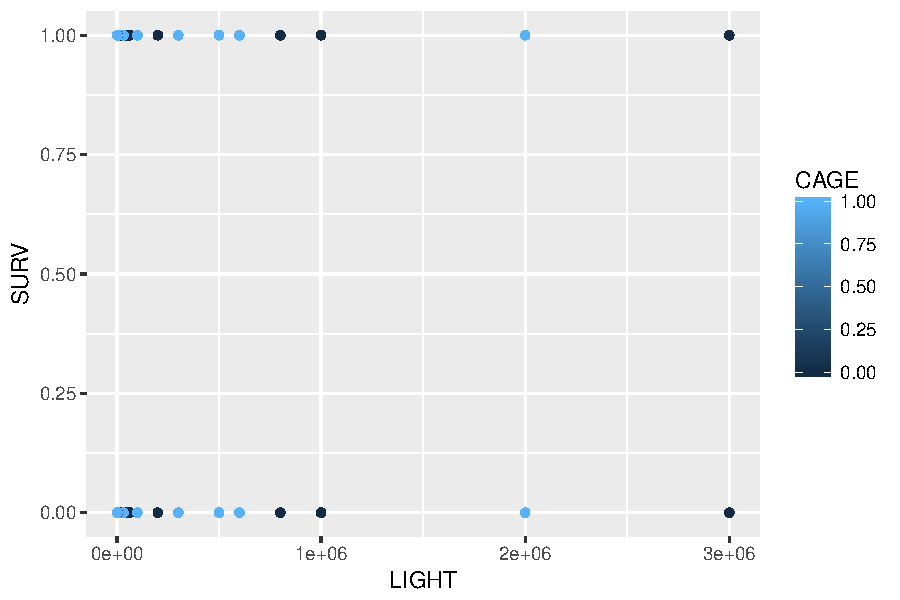
\includegraphics[width=\maxwidth]{figure/unnamed-chunk-3-1} 

}



\end{knitrout}

\end{frame}


\begin{frame}  \frametitle{Boosting}
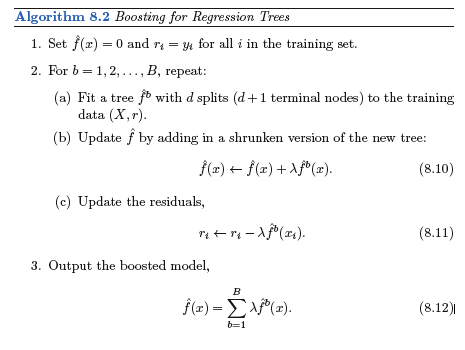
\includegraphics[height=3in]{boostingAlgo}

\end{frame}

\begin{frame}
  \frametitle{Boosting }
  \begin{itemize}
  \item Mean is a sum of B trees  \pause
  \item Boosting can over-fit if $B$ is too large  \pause
  \item The number of splits, $d$, in each tree controls  the complexity of the boosted ensemble; $d = 1$ corresponds to models of stumps  \pause
\item $d$ is the interaction depth; $d$ splits can involve $d$ variables.  (default in {\tt gbm} package is $4$)  \pause
  \end{itemize}
\end{frame}


\begin{frame}[fragile]  \frametitle{Boosting Example}
\begin{knitrout}
\definecolor{shadecolor}{rgb}{0.969, 0.969, 0.969}\color{fgcolor}\begin{kframe}
\begin{alltt}
\hlkwd{suppressMessages}\hlstd{(}\hlkwd{library}\hlstd{(gbm))}
\hlstd{boost.car} \hlkwb{=}\hlkwd{gbm}\hlstd{(}\hlkwd{I}\hlstd{(}\hlkwd{as.numeric}\hlstd{(High)}\hlopt{-}\hlnum{1}\hlstd{)} \hlopt{~} \hlstd{.} \hlopt{-}\hlstd{Sales,}
               \hlkwc{data}\hlstd{=Carseats[train ,],}
               \hlkwc{distribution}\hlstd{=}\hlstr{"bernoulli"}\hlstd{,}
               \hlkwc{n.trees} \hlstd{=}\hlnum{5000}\hlstd{,} \hlkwc{interaction.depth} \hlstd{=}\hlnum{4}\hlstd{)}
\hlstd{yhat.boost} \hlkwb{=} \hlkwd{ifelse}\hlstd{(}\hlkwd{predict}\hlstd{(boost.car,}
                      \hlkwc{newdata}\hlstd{=Carseats.test,}
                      \hlkwc{n.trees}\hlstd{=}\hlnum{5000}\hlstd{,}
                      \hlkwc{type}\hlstd{=}\hlstr{"response"}\hlstd{)} \hlopt{>} \hlnum{.5}\hlstd{,} \hlnum{1}\hlstd{,} \hlnum{0}\hlstd{)}
\hlstd{tab} \hlkwb{=}\hlkwd{table}\hlstd{(yhat.boost, Carseats.test}\hlopt{$}\hlstd{High)}
\hlstd{tab} \hlkwb{=} \hlkwd{table}\hlstd{(yhat.boost,Carseats.test}\hlopt{$}\hlstd{High)}
\hlstd{tab}
\end{alltt}
\begin{verbatim}
##           
## yhat.boost  No Yes 
##          0 100   16
##          1  16   68
\end{verbatim}
\begin{alltt}
\hlstd{CE.tab[}\hlstr{"Boosting"}\hlstd{,} \hlnum{1}\hlstd{]}\hlkwb{=} \hlstd{(tab[}\hlnum{1}\hlstd{,}\hlnum{1}\hlstd{]} \hlopt{+} \hlstd{tab[}\hlnum{2}\hlstd{,}\hlnum{2}\hlstd{])}\hlopt{/}\hlkwd{sum}\hlstd{(tab)}

\hlstd{CE.tab[}\hlstr{"Boosting"}\hlstd{,]}
\end{alltt}
\begin{verbatim}
## [1] 0.84
\end{verbatim}
\end{kframe}
\end{knitrout}

84.5\% accuracy!
\end{frame}

\begin{frame}[fragile]  \frametitle{Variable Importance: Boosting}
\begin{knitrout}
\definecolor{shadecolor}{rgb}{0.969, 0.969, 0.969}\color{fgcolor}\begin{kframe}
\begin{alltt}
\hlkwd{summary}\hlstd{(boost.car,} \hlkwc{plotit}\hlstd{=}\hlnum{FALSE}\hlstd{)}
\end{alltt}
\begin{verbatim}
##                     var    rel.inf
## Price             Price 27.1860994
## ShelveLoc     ShelveLoc 20.9558458
## Advertising Advertising 14.3652543
## Age                 Age 13.0972300
## CompPrice     CompPrice  8.6307712
## Income           Income  6.6391956
## Population   Population  6.1235720
## Education     Education  1.6769694
## Urban             Urban  0.8472994
## US                   US  0.4777628
\end{verbatim}
\end{kframe}
\end{knitrout}
\end{frame}

\begin{frame}[fragile] \frametitle{Variable Importance: summary(boost.car)}
\begin{knitrout}
\definecolor{shadecolor}{rgb}{0.969, 0.969, 0.969}\color{fgcolor}

{\centering 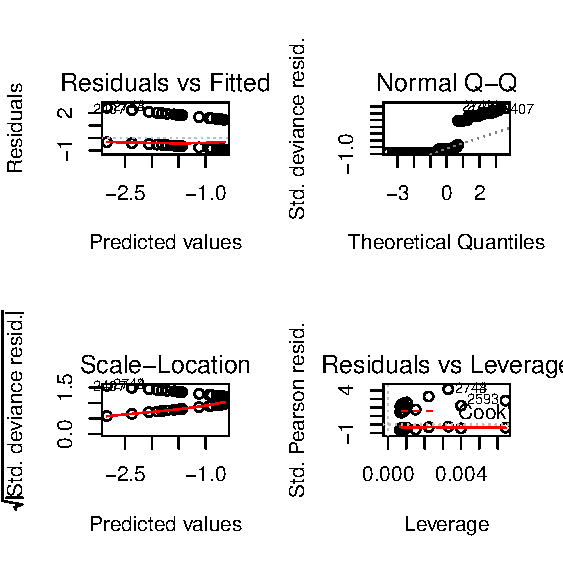
\includegraphics[width=\maxwidth]{figure/unnamed-chunk-6-1} 

}


\begin{kframe}\begin{verbatim}
##                     var    rel.inf
## Price             Price 27.1860994
## ShelveLoc     ShelveLoc 20.9558458
## Advertising Advertising 14.3652543
## Age                 Age 13.0972300
## CompPrice     CompPrice  8.6307712
## Income           Income  6.6391956
## Population   Population  6.1235720
## Education     Education  1.6769694
## Urban             Urban  0.8472994
## US                   US  0.4777628
\end{verbatim}
\end{kframe}
\end{knitrout}
\end{frame}


\begin{frame}
  \frametitle{Bayesian Additive Regression Trees}
Gaussian Model:  Single Tree model

$$
Y = g(x, T, M) + \eps
$$
Where $T$ is a tree and $M= (\mu_1, \ldots \mu_b)^T$ is the vector of means at the terminal nodes of the tree given by $T$  \pause

\vspace{12pt}
BART represents the mean function as

$$
Y =\sum_j  g(x, T_j, M_j) + \eps
$$
as a sum of trees. \pause


Priors control the complexity of each tree; back-fitting as in boosting. \pause

\end{frame}


\begin{frame}[fragile] \frametitle{BART: Bayesian Additive Regression Trees}
\begin{knitrout}
\definecolor{shadecolor}{rgb}{0.969, 0.969, 0.969}\color{fgcolor}\begin{kframe}
\begin{alltt}
\hlkwd{library}\hlstd{(BayesTree)}
\end{alltt}


{\ttfamily\noindent\bfseries\color{errorcolor}{\#\# Error in library(BayesTree): there is no package called 'BayesTree'}}\begin{alltt}
\hlkwd{set.seed}\hlstd{(}\hlnum{42}\hlstd{)}
\hlstd{bart.carseats} \hlkwb{=} \hlkwd{bart}\hlstd{(}\hlkwc{x.train}\hlstd{=Carseats[train,}\hlopt{-}\hlkwd{c}\hlstd{(}\hlnum{1}\hlstd{,}\hlnum{12}\hlstd{)],}
                   \hlkwc{y.train}\hlstd{=Carseats}\hlopt{$}\hlstd{High[train],}
                   \hlkwc{x.test}\hlstd{=Carseats[}\hlopt{-}\hlstd{train,}\hlopt{-}\hlkwd{c}\hlstd{(}\hlnum{1}\hlstd{,}\hlnum{12}\hlstd{)],}
                   \hlkwc{verbose}\hlstd{=}\hlnum{FALSE}   \hlstd{)}
\end{alltt}


{\ttfamily\noindent\bfseries\color{errorcolor}{\#\# Error in eval(expr, envir, enclos): could not find function "{}bart"{}}}\begin{alltt}
\hlstd{pihat.bart} \hlkwb{=} \hlkwd{apply}\hlstd{(}\hlkwd{pnorm}\hlstd{(bart.carseats}\hlopt{$}\hlstd{yhat.test),} \hlnum{2}\hlstd{, mean)}
\end{alltt}


{\ttfamily\noindent\bfseries\color{errorcolor}{\#\# Error in pnorm(bart.carseats\$yhat.test): object 'bart.carseats' not found}}\begin{alltt}
\hlstd{yhat.bart} \hlkwb{=} \hlkwd{ifelse}\hlstd{(pihat.bart} \hlopt{>} \hlnum{.5}\hlstd{,} \hlnum{1}\hlstd{,} \hlnum{0}\hlstd{)}
\end{alltt}


{\ttfamily\noindent\bfseries\color{errorcolor}{\#\# Error in ifelse(pihat.bart > 0.5, 1, 0): object 'pihat.bart' not found}}\begin{alltt}
\hlstd{tab} \hlkwb{=} \hlkwd{table}\hlstd{(yhat.bart, Carseats.test}\hlopt{$}\hlstd{High)}
\end{alltt}


{\ttfamily\noindent\bfseries\color{errorcolor}{\#\# Error in table(yhat.bart, Carseats.test\$High): object 'yhat.bart' not found}}\begin{alltt}
\hlstd{CE.tab[}\hlstr{"BART"}\hlstd{,} \hlnum{1}\hlstd{]}\hlkwb{=} \hlstd{(tab[}\hlnum{1}\hlstd{,}\hlnum{1}\hlstd{]} \hlopt{+} \hlstd{tab[}\hlnum{2}\hlstd{,}\hlnum{2}\hlstd{])}\hlopt{/}\hlkwd{sum}\hlstd{(tab)}

\hlstd{CE.tab[}\hlstr{"BART"}\hlstd{,]}
\end{alltt}
\begin{verbatim}
## [1] 0.84
\end{verbatim}
\begin{alltt}
\hlcom{#> investigate_var_importance(bart.carseats)}
\end{alltt}
\end{kframe}
\end{knitrout}
\end{frame}

\begin{frame} \frametitle{Uncertainty in Mean Function}
\begin{knitrout}
\definecolor{shadecolor}{rgb}{0.969, 0.969, 0.969}\color{fgcolor}\begin{kframe}
\begin{alltt}
\hlkwd{plot}\hlstd{(bart.carseats)}
\end{alltt}


{\ttfamily\noindent\bfseries\color{errorcolor}{\#\# Error in plot(bart.carseats): object 'bart.carseats' not found}}\end{kframe}
\end{knitrout}
\end{frame}

\begin{frame}[fragile] \frametitle{Partial Dependendence (computationally intensive!)}
\begin{knitrout}
\definecolor{shadecolor}{rgb}{0.969, 0.969, 0.969}\color{fgcolor}

{\centering \includegraphics[width=\maxwidth]{figure/unnamed-chunk-9-1} 

}



\end{knitrout}

\end{frame}

\begin{frame}[fragile] \frametitle{BartMachine}
\begin{knitrout}
\definecolor{shadecolor}{rgb}{0.969, 0.969, 0.969}\color{fgcolor}\begin{kframe}
\begin{alltt}
\hlkwd{suppressMessages}\hlstd{(}\hlkwd{library}\hlstd{(bartMachine))}
\hlkwd{set.seed}\hlstd{(}\hlnum{42}\hlstd{)}
\hlstd{bart.carseats} \hlkwb{=} \hlkwd{bartMachine}\hlstd{(}\hlkwc{X}\hlstd{=Carseats[train,}\hlopt{-}\hlkwd{c}\hlstd{(}\hlnum{1}\hlstd{,}\hlnum{12}\hlstd{)],}
                            \hlkwc{y}\hlstd{=Carseats}\hlopt{$}\hlstd{High[train],}
                            \hlkwc{verb}\hlstd{=}\hlnum{FALSE}\hlstd{,} \hlkwc{serialize}\hlstd{=}\hlnum{TRUE}\hlstd{)}
\end{alltt}
\begin{verbatim}
## serializing in order to be saved for future R sessions...done
\end{verbatim}
\begin{alltt}
\hlstd{yhat.bart} \hlkwb{=} \hlkwd{predict}\hlstd{(bart.carseats,}
                    \hlstd{Carseats.test[,} \hlopt{-}\hlkwd{c}\hlstd{(}\hlnum{1}\hlstd{,}\hlnum{12}\hlstd{)],}
                    \hlkwc{type}\hlstd{=}\hlstr{"class"}\hlstd{)}
\hlkwd{table}\hlstd{(yhat.bart, Carseats.test}\hlopt{$}\hlstd{High)}
\end{alltt}
\begin{verbatim}
##          
## yhat.bart  No Yes 
##      No   103   20
##      Yes   13   64
\end{verbatim}
\end{kframe}
\end{knitrout}

\end{frame}

\begin{frame}[fragile]\frametitle{Variable Importance}
\begin{knitrout}
\definecolor{shadecolor}{rgb}{0.969, 0.969, 0.969}\color{fgcolor}\begin{kframe}


{\ttfamily\noindent\bfseries\color{errorcolor}{\#\# Error in library(bartMachine): there is no package called 'bartMachine'}}\end{kframe}
\end{knitrout}

\begin{knitrout}
\definecolor{shadecolor}{rgb}{0.969, 0.969, 0.969}\color{fgcolor}\begin{kframe}
\begin{alltt}
\hlkwd{investigate_var_importance}\hlstd{(bart.carseats)}
\end{alltt}


{\ttfamily\noindent\bfseries\color{errorcolor}{\#\# Error in eval(expr, envir, enclos): could not find function "{}investigate\_var\_importance"{}}}\end{kframe}
\end{knitrout}
\end{frame}

\begin{frame}[fragile]\frametitle{GLMs and Bayesian Variable Selection}
\begin{knitrout}
\definecolor{shadecolor}{rgb}{0.969, 0.969, 0.969}\color{fgcolor}\begin{kframe}
\begin{alltt}
\hlkwd{set.seed}\hlstd{(}\hlnum{42}\hlstd{);} \hlkwd{library}\hlstd{(BAS)}
\hlstd{bas.carseats} \hlkwb{=} \hlkwd{bas.glm}\hlstd{(High} \hlopt{~} \hlstd{.} \hlopt{-} \hlstd{Sales,} \hlkwc{data}\hlstd{=Carseats,}
                       \hlkwc{subset}\hlstd{=train,} \hlkwc{family}\hlstd{=}\hlkwd{binomial}\hlstd{(),}
                       \hlkwc{method}\hlstd{=}\hlstr{"MCMC"}\hlstd{,}  \hlkwc{n.models}\hlstd{=}\hlnum{10000}\hlstd{,}
                       \hlkwc{betaprior}\hlstd{=}\hlkwd{bic.prior}\hlstd{(}\hlkwc{n}\hlstd{=}\hlnum{200}\hlstd{))}
\hlstd{yhat} \hlkwb{=} \hlkwd{predict}\hlstd{(bas.carseats,} \hlkwc{newdata}\hlstd{=Carseats[}\hlopt{-}\hlstd{train,])}
\hlstd{tab} \hlkwb{=} \hlkwd{table}\hlstd{(}\hlkwd{ifelse}\hlstd{(yhat}\hlopt{$}\hlstd{fit} \hlopt{>} \hlnum{.5}\hlstd{,} \hlnum{1}\hlstd{,} \hlnum{0}\hlstd{), Carseats.test}\hlopt{$}\hlstd{High)}
\hlstd{CE.tab[}\hlstr{"BMA"}\hlstd{,} \hlnum{1}\hlstd{]}\hlkwb{=} \hlstd{(tab[}\hlnum{1}\hlstd{,}\hlnum{1}\hlstd{]} \hlopt{+} \hlstd{tab[}\hlnum{2}\hlstd{,}\hlnum{2}\hlstd{])}\hlopt{/}\hlkwd{sum}\hlstd{(tab)}

\hlstd{CE.tab[}\hlstr{"BMA"}\hlstd{,]}
\end{alltt}
\begin{verbatim}
## [1] 0.905
\end{verbatim}
\begin{alltt}
\hlcom{#(107 + 74)/200}
\end{alltt}
\end{kframe}
\end{knitrout}
\end{frame}

\begin{frame}[fragile]\frametitle{LASSO Variable Selection}
\begin{knitrout}
\definecolor{shadecolor}{rgb}{0.969, 0.969, 0.969}\color{fgcolor}\begin{kframe}
\begin{alltt}
\hlkwd{set.seed}\hlstd{(}\hlnum{42}\hlstd{);} \hlkwd{library}\hlstd{(glmnet)}
\end{alltt}


{\ttfamily\noindent\itshape\color{messagecolor}{\#\# Loading required package: Matrix}}

{\ttfamily\noindent\itshape\color{messagecolor}{\#\# Loading required package: foreach}}

{\ttfamily\noindent\itshape\color{messagecolor}{\#\# Loaded glmnet 2.0-5}}\begin{alltt}
\hlstd{glmnet.carseats} \hlkwb{=} \hlkwd{cv.glmnet}\hlstd{(}
  \hlkwc{x}\hlstd{=}\hlkwd{model.matrix}\hlstd{(High} \hlopt{~} \hlstd{.} \hlopt{-} \hlstd{Sales,} \hlkwc{data}\hlstd{=Carseats[train,]),}
  \hlkwc{y}\hlstd{=(}\hlkwd{as.numeric}\hlstd{(Carseats}\hlopt{$}\hlstd{High[train])} \hlopt{-} \hlnum{1}\hlstd{),} \hlkwc{family}\hlstd{=}\hlstr{"binomial"}\hlstd{)}
\hlstd{yhat} \hlkwb{=} \hlkwd{predict}\hlstd{(glmnet.carseats,}
               \hlkwc{newx}\hlstd{=}\hlkwd{model.matrix}\hlstd{(High} \hlopt{~} \hlstd{.} \hlopt{-} \hlstd{Sales,} \hlkwc{data}\hlstd{=Carseats[}\hlopt{-}\hlstd{train,]))}
\hlstd{tab} \hlkwb{=} \hlkwd{table}\hlstd{(}\hlkwd{ifelse}\hlstd{(yhat} \hlopt{>} \hlnum{.0}\hlstd{,} \hlnum{1}\hlstd{,} \hlnum{0}\hlstd{), Carseats.test}\hlopt{$}\hlstd{High)}
\hlstd{CE.tab[}\hlstr{"LASSO"}\hlstd{,} \hlnum{1}\hlstd{]}\hlkwb{=} \hlstd{(tab[}\hlnum{1}\hlstd{,}\hlnum{1}\hlstd{]} \hlopt{+} \hlstd{tab[}\hlnum{2}\hlstd{,}\hlnum{2}\hlstd{])}\hlopt{/}\hlkwd{sum}\hlstd{(tab)}

\hlstd{CE.tab[}\hlstr{"LASSO"}\hlstd{,]}
\end{alltt}
\begin{verbatim}
## [1] 0.89
\end{verbatim}
\end{kframe}
\end{knitrout}
\end{frame}
\begin{frame}\frametitle{Summary}
  \begin{itemize}
  \item Trees are simple to understand, but have high variability \pause
  \item Bagging (Averaging) reduces variability \pause
  \item Random Forests adds additional constraints to average trees
    that are different (reduced correlation leads to reduction in variance). \pause
  \item Boosting builds a mean function that uses multiple trees where
    the growth takes into account the previous trees.  Smaller trees
    can be used  (larger trees can overfit) \pause
\item BART is similar to Boosting in that the mean function is a sum
  of trees, but uses a Bayesian approach to control complexity.  Trees
  can be of different sizes and the number of trees can be large without overfitting \pause

\item Plots may suggest that a (generalized) linear model  may be appropriate! \pause

  \end{itemize}
Interpretability? For which methods can you explain how changes in a predictor change the response?
\end{frame}
\begin{knitrout}
\definecolor{shadecolor}{rgb}{0.969, 0.969, 0.969}\color{fgcolor}\begin{kframe}
\begin{alltt}
\hlkwd{save}\hlstd{(CE.tab,} \hlkwc{file}\hlstd{=}\hlstr{"OoS.accuracy"}\hlstd{)}
\end{alltt}
\end{kframe}
\end{knitrout}

\end{document}
